% classnames = {'wave2','balance','bend','box','clap','dance','wave1'};
\begin{figure*}[*th] 
\begin{center}
{\footnotesize
\begin{tabular}{@{}c@{}c@{}c@{}c@{}c@{}c@{}c@{}c@{}} 
\rotatebox{90}{\hspace{3mm}\textbf{(a) Balance}}
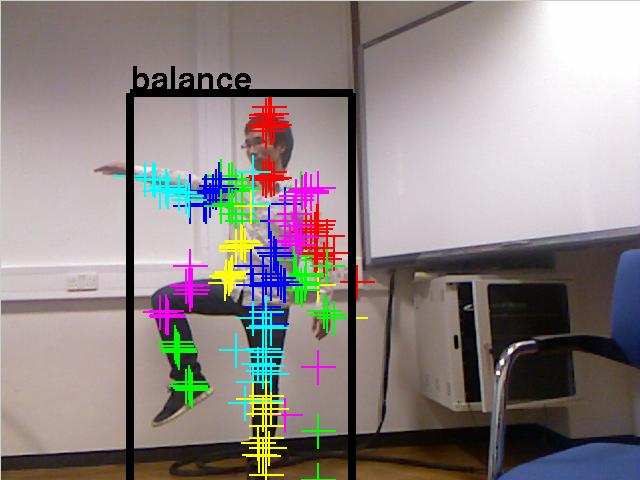
\includegraphics[height=0.11\linewidth]{fig/poseest/APE/balc.jpg} 
&
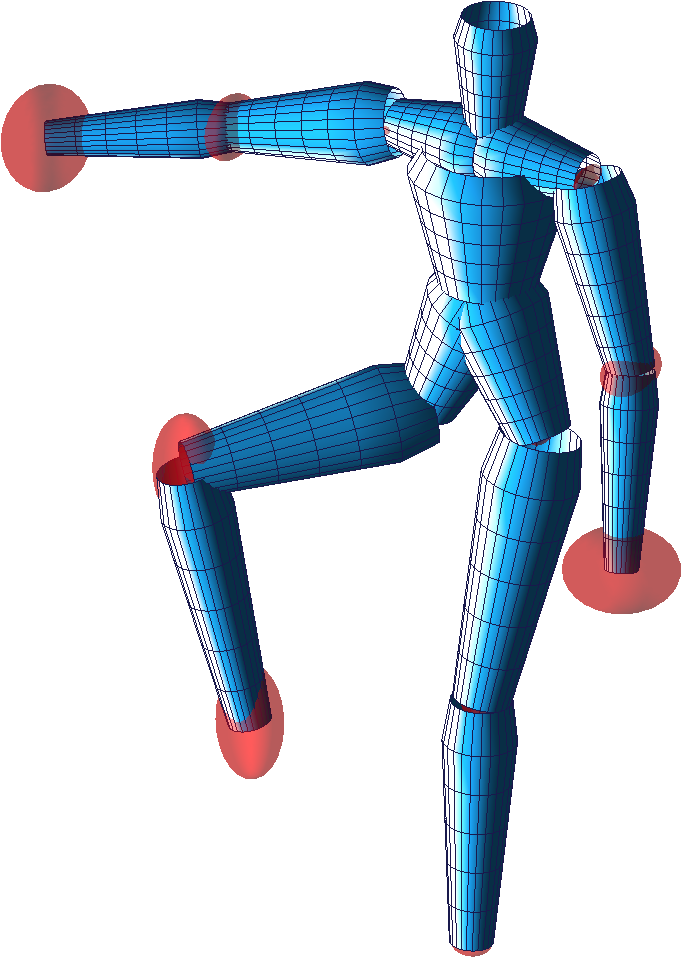
\includegraphics[height=0.135\linewidth]{fig/poseest/APE/balc.png}
& 
\rotatebox{90}{\hspace{3mm}\textbf{(b) Balance}}
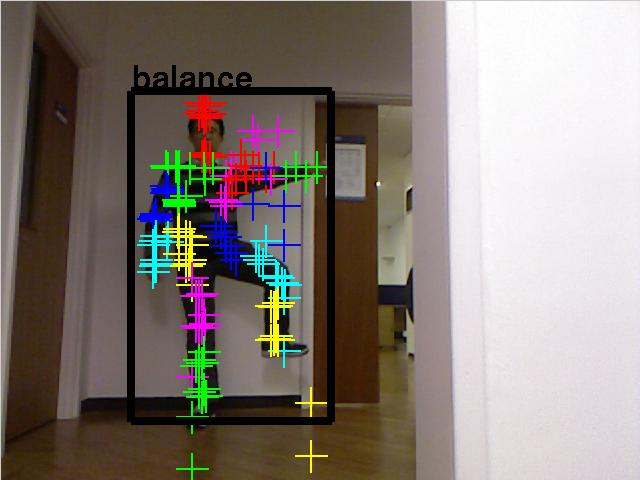
\includegraphics[height=0.11\linewidth]{fig/poseest/APE/balc2.jpg} 
&
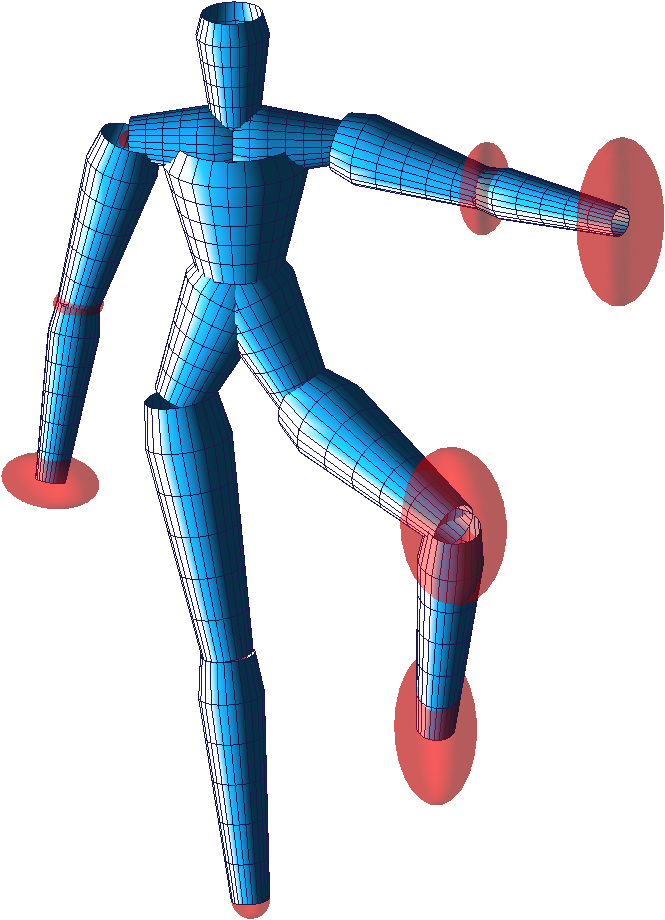
\includegraphics[height=0.135\linewidth]{fig/poseest/APE/balc2.png}
& 
\rotatebox{90}{\hspace{3mm}\textbf{(c) Bend}}
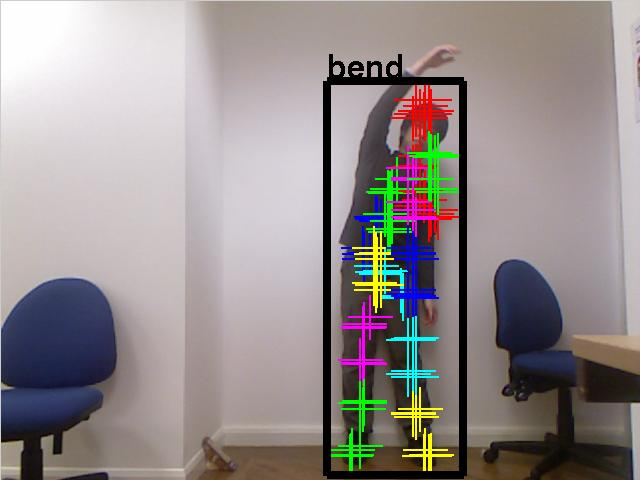
\includegraphics[height=0.11\linewidth]{fig/poseest/APE/bend.jpg} 
&
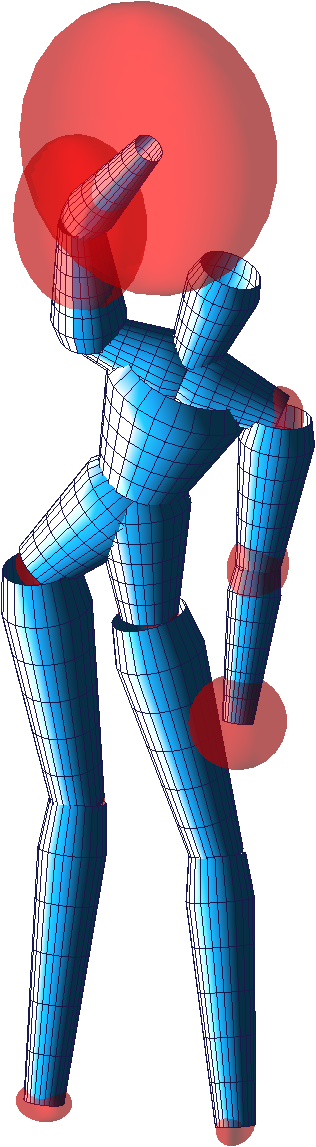
\includegraphics[height=0.135\linewidth]{fig/poseest/APE/bend.png}
& 
\rotatebox{90}{\hspace{3mm}\textbf{(d) Bend}}
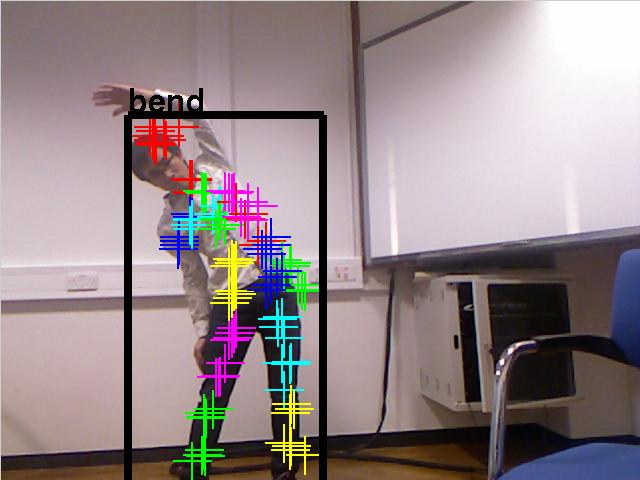
\includegraphics[height=0.11\linewidth]{fig/poseest/APE/bend2.jpg} 
&
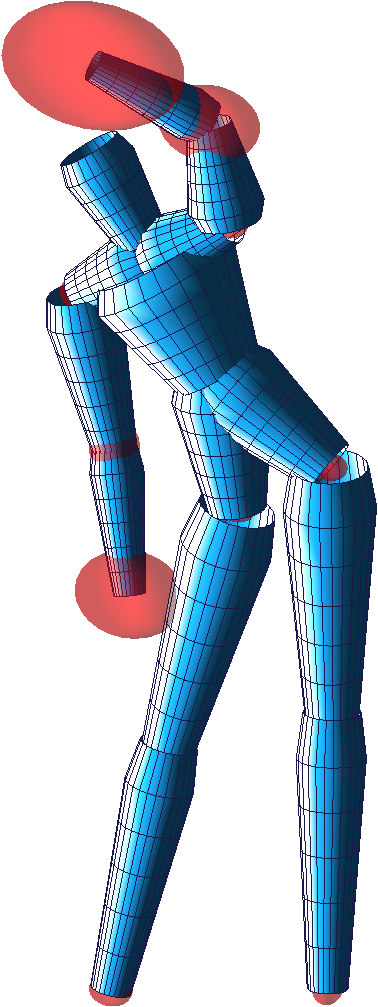
\includegraphics[height=0.135\linewidth]{fig/poseest/APE/bend2.png}
\\
\rotatebox{90}{\hspace{3mm}\textbf{(e) Box}}
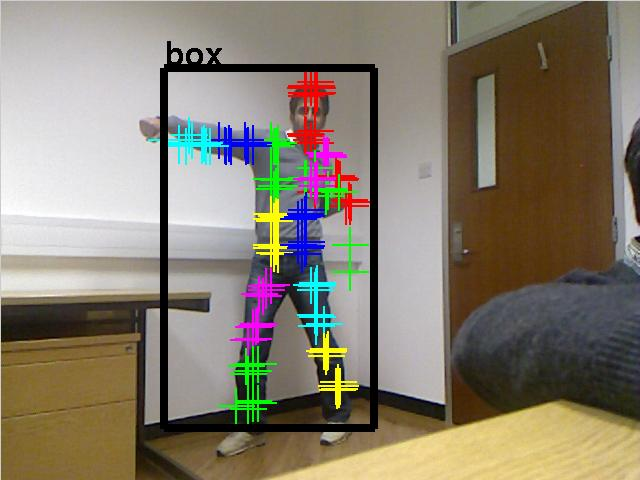
\includegraphics[height=0.11\linewidth]{fig/poseest/APE/boxx.jpg} 
&
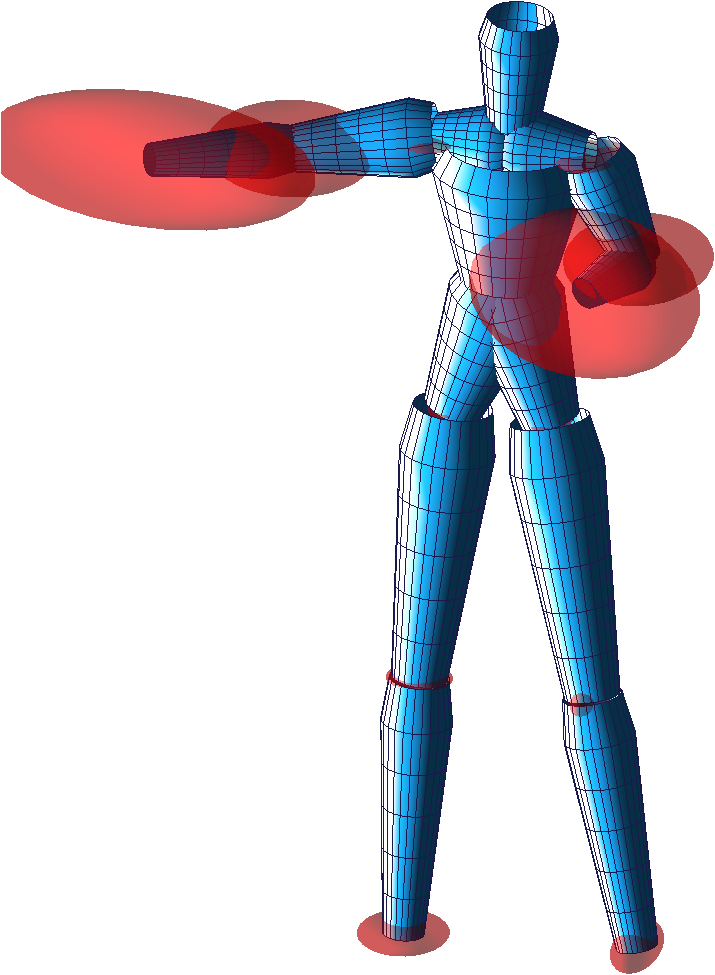
\includegraphics[height=0.135\linewidth]{fig/poseest/APE/boxx.png}
& 
\rotatebox{90}{\hspace{3mm}\textbf{(f) Box}}
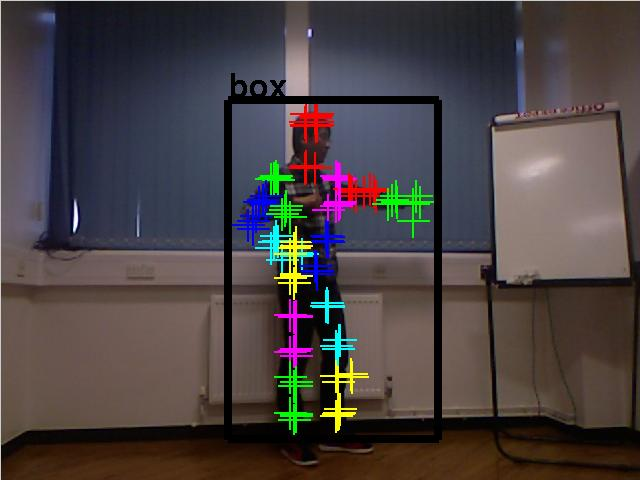
\includegraphics[height=0.11\linewidth]{fig/poseest/APE/boxx2.jpg} 
&
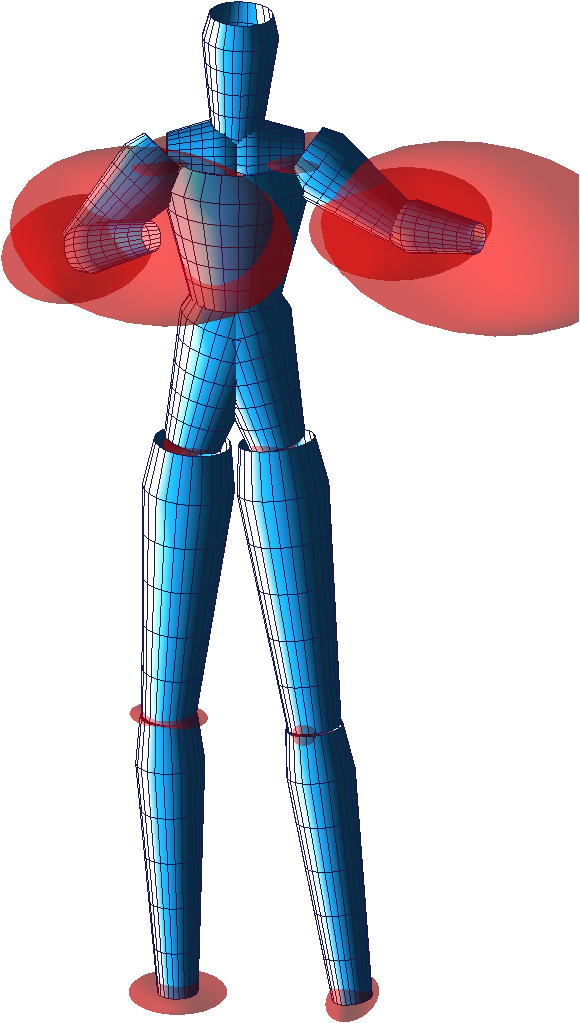
\includegraphics[height=0.135\linewidth]{fig/poseest/APE/boxx2.png}
& 
\rotatebox{90}{\hspace{3mm}\textbf{(g) Clap}}
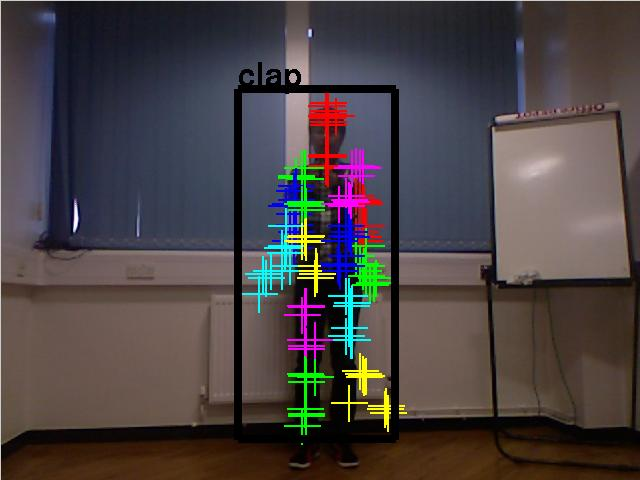
\includegraphics[height=0.11\linewidth]{fig/poseest/APE/clap.jpg} 
&
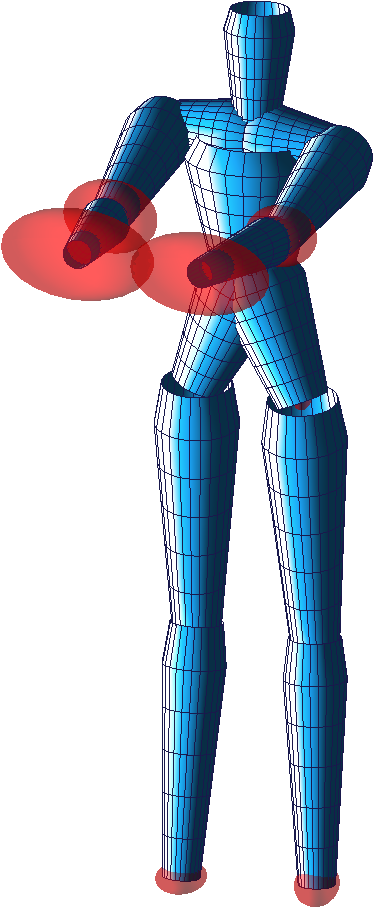
\includegraphics[height=0.135\linewidth]{fig/poseest/APE/clap.png}
& 
\rotatebox{90}{\hspace{3mm}\textbf{(h) Clap}}
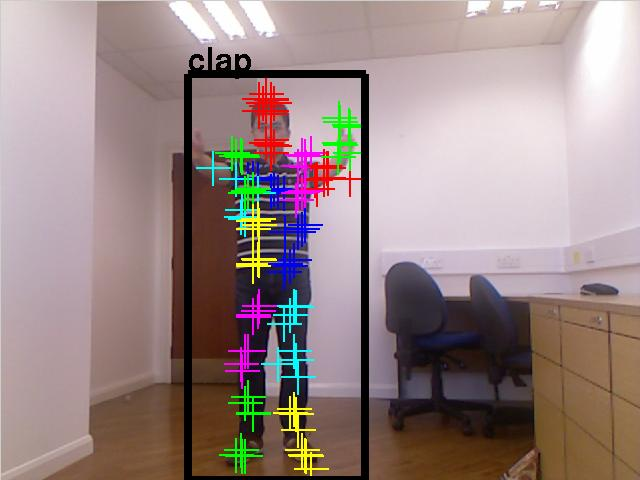
\includegraphics[height=0.11\linewidth]{fig/poseest/APE/clap2.jpg} 
&
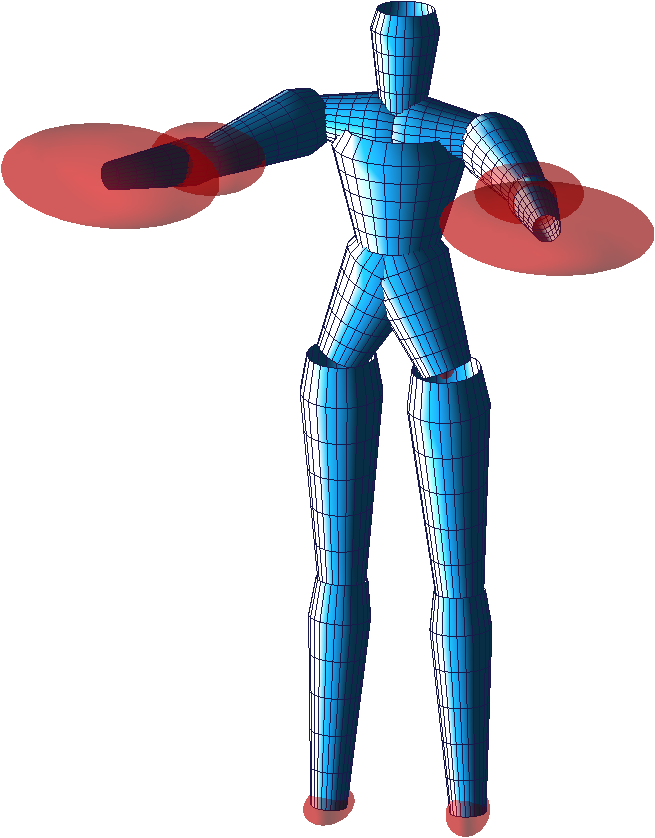
\includegraphics[height=0.135\linewidth]{fig/poseest/APE/clap2.png}
\\
\rotatebox{90}{\hspace{3mm}\textbf{(i) Dance}}
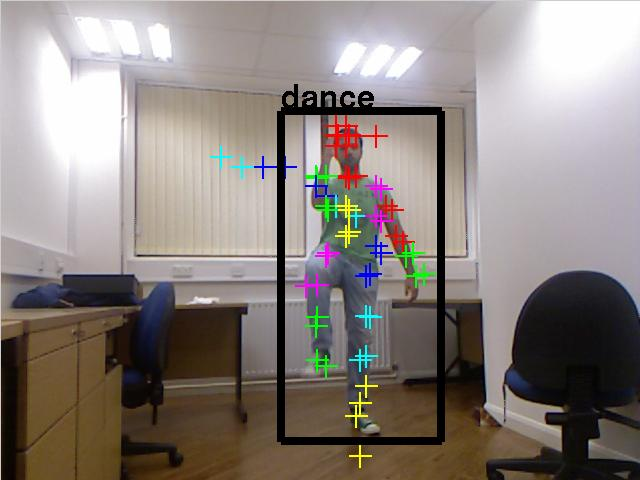
\includegraphics[height=0.11\linewidth]{fig/poseest/APE/dance.jpg} 
&
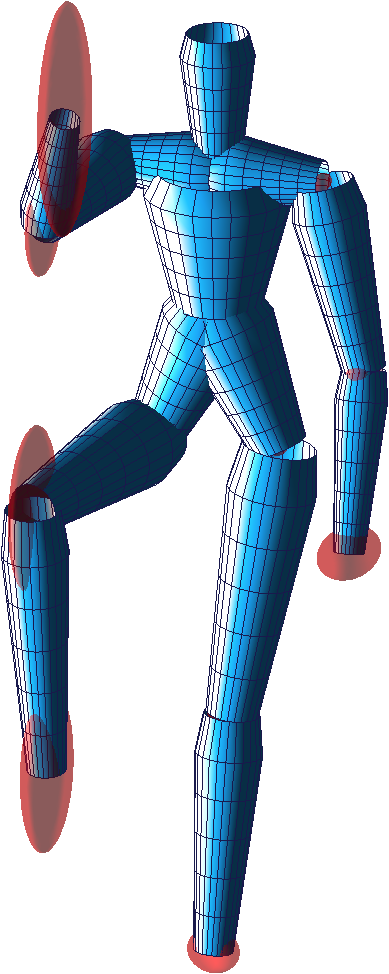
\includegraphics[height=0.135\linewidth]{fig/poseest/APE/dance.png}
& 
\rotatebox{90}{\hspace{3mm}\textbf{(j) Dance}}
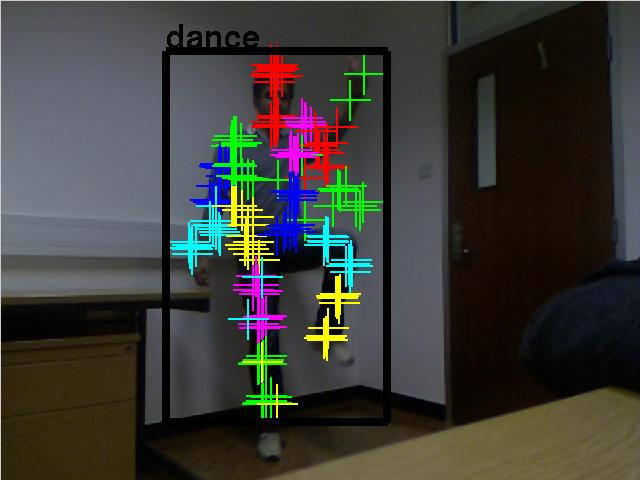
\includegraphics[height=0.11\linewidth]{fig/poseest/APE/dance2.jpg} 
&
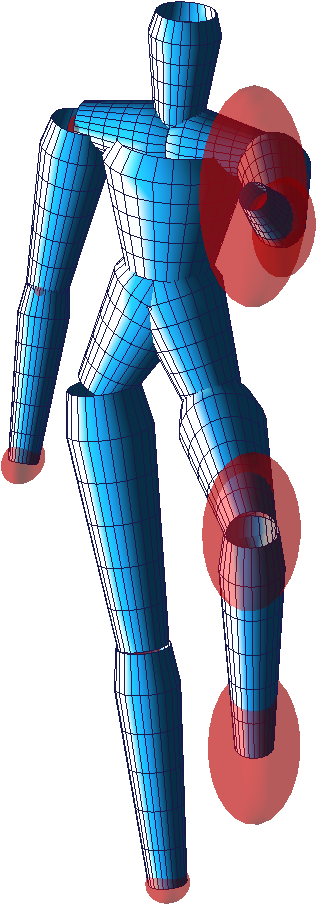
\includegraphics[height=0.135\linewidth]{fig/poseest/APE/dance2.png}
& 
\rotatebox{90}{\hspace{3mm}\textbf{(k) Wave 1}}
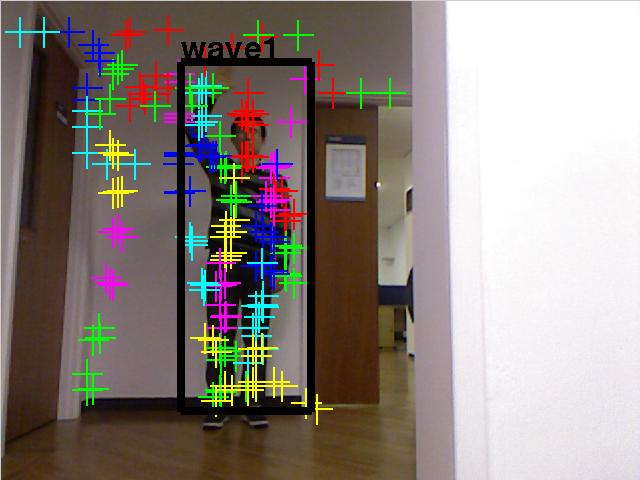
\includegraphics[height=0.11\linewidth]{fig/poseest/APE/wave1.jpg} 
&
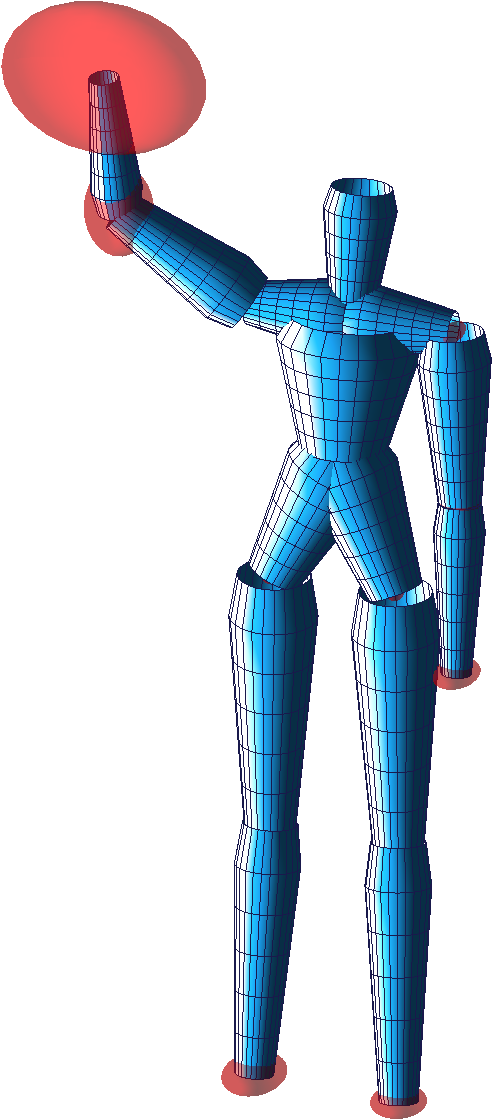
\includegraphics[height=0.135\linewidth]{fig/poseest/APE/wave1.png}
& 
\rotatebox{90}{\hspace{3mm}\textbf{(l) Wave 1}}
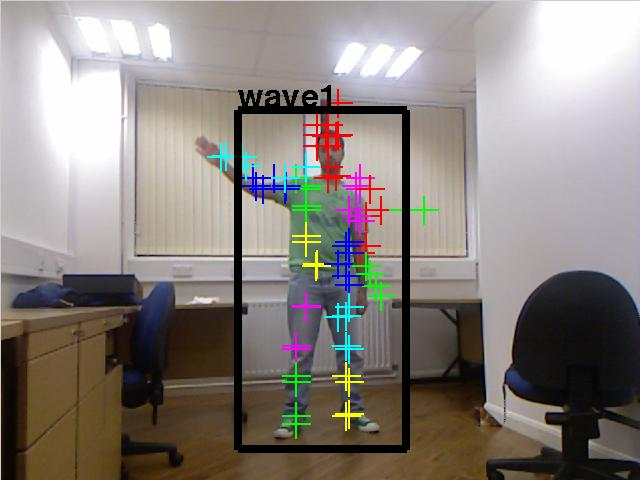
\includegraphics[height=0.11\linewidth]{fig/poseest/APE/wave12.jpg} 
&
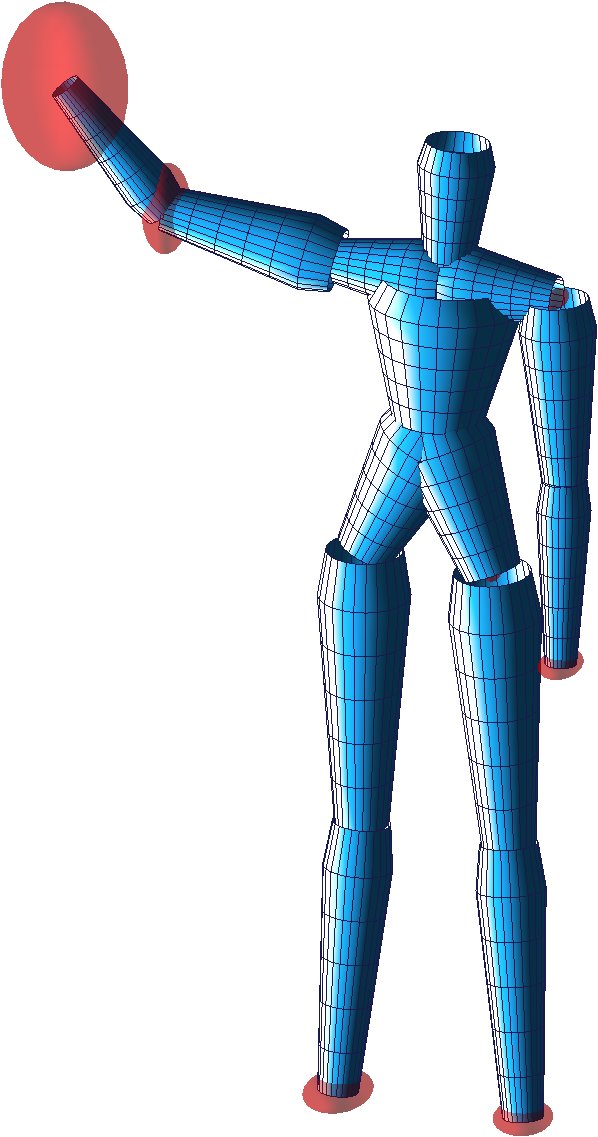
\includegraphics[height=0.135\linewidth]{fig/poseest/APE/wave12.png}
\\
\rotatebox{90}{\hspace{3mm}\textbf{(m) Wave 2}}
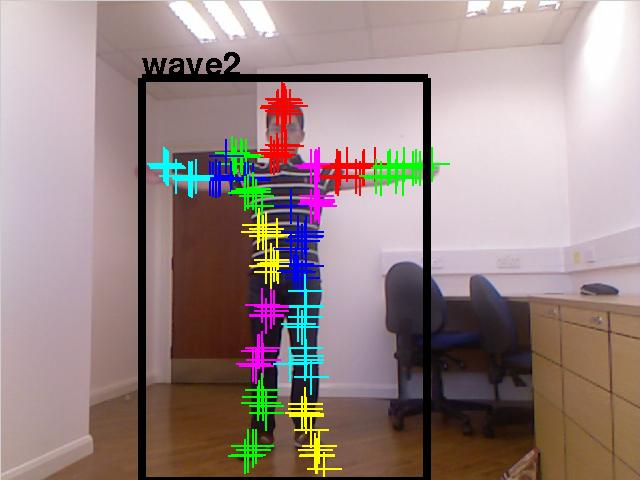
\includegraphics[height=0.11\linewidth]{fig/poseest/APE/wave2.jpg} 
&
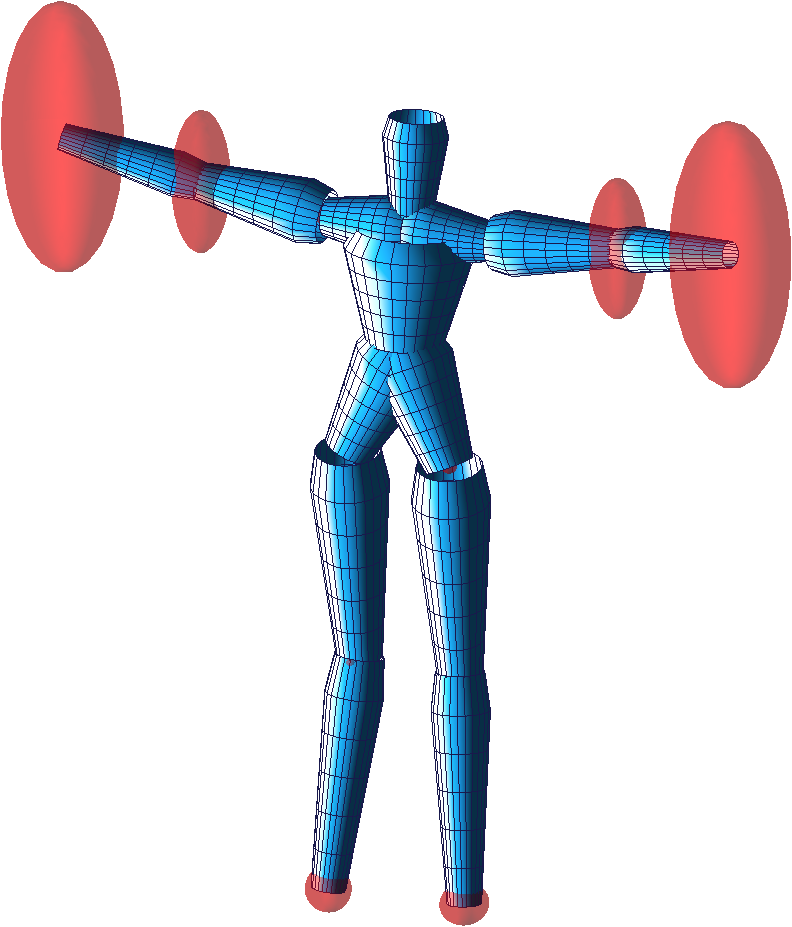
\includegraphics[height=0.135\linewidth]{fig/poseest/APE/wave2.png}
& 
\rotatebox{90}{\hspace{3mm}\textbf{(n) Wave 2}}
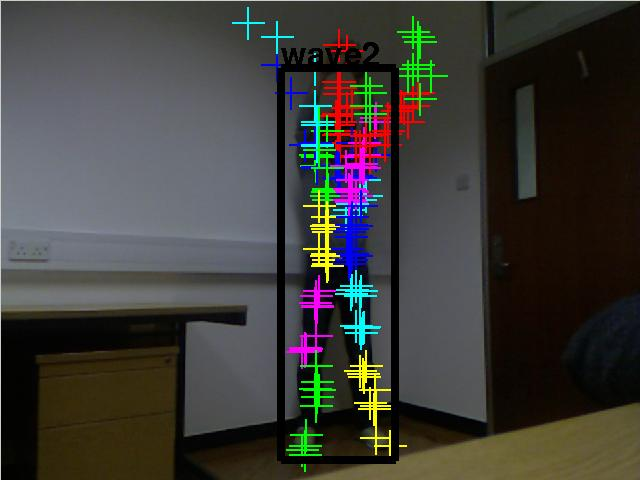
\includegraphics[height=0.11\linewidth]{fig/poseest/APE/wave22.jpg} 
&
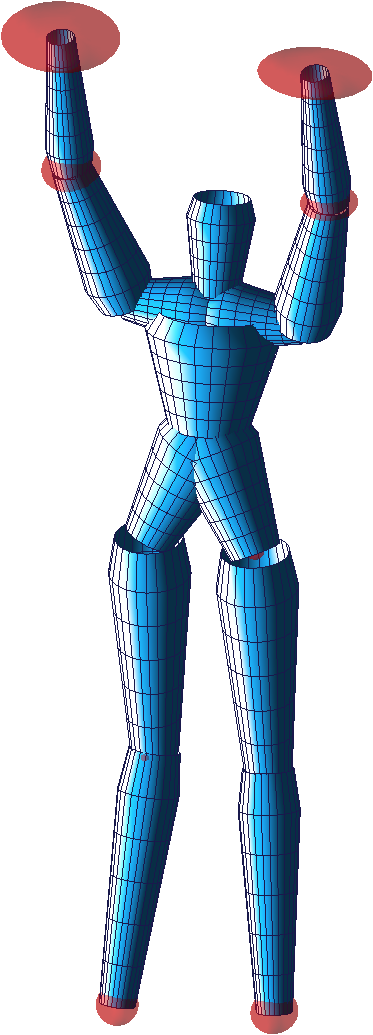
\includegraphics[height=0.135\linewidth]{fig/poseest/APE/wave22.png}
& 
\rotatebox{90}{\hspace{3mm}\textbf{(o) Bend}}
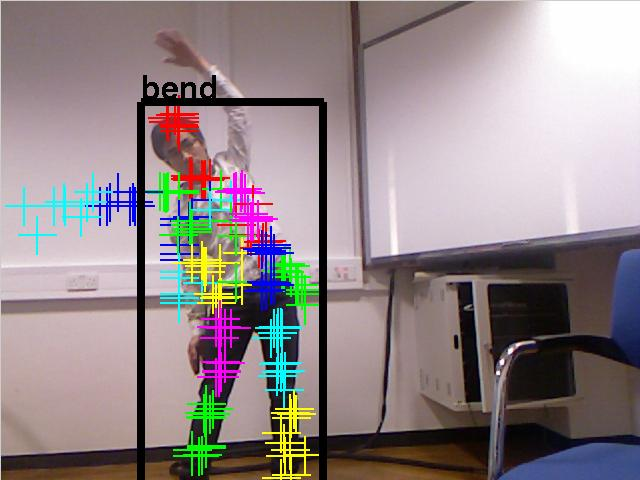
\includegraphics[height=0.11\linewidth]{fig/poseest/APE/benderr.jpg} 
&
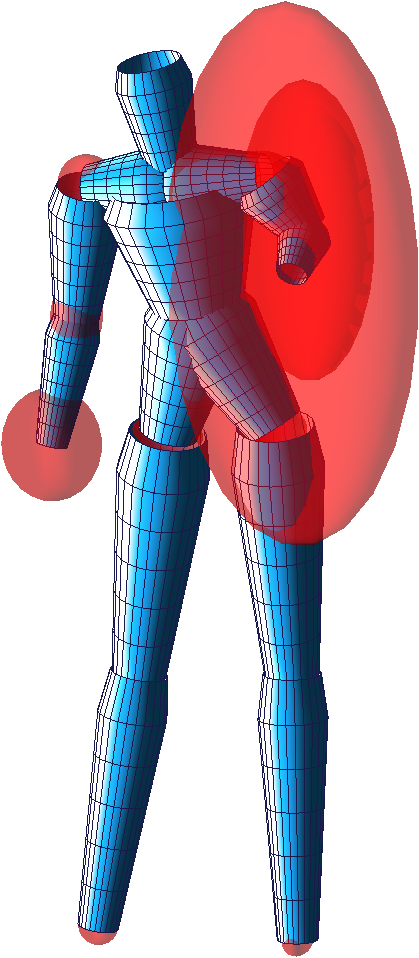
\includegraphics[height=0.135\linewidth]{fig/poseest/APE/benderr.png}
& 
\rotatebox{90}{\hspace{3mm}\textbf{(p) Box}}
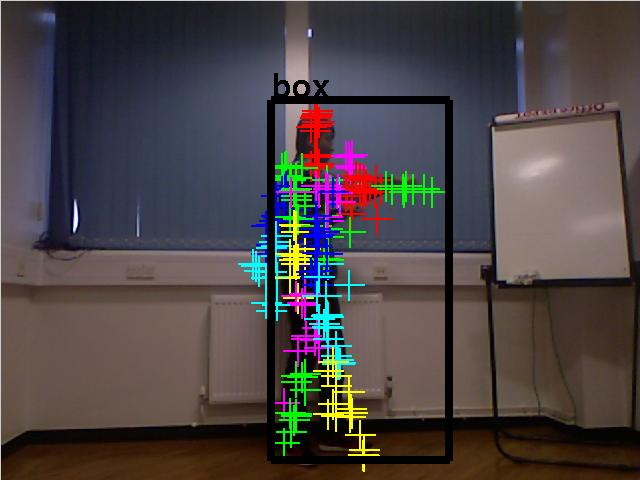
\includegraphics[height=0.11\linewidth]{fig/poseest/APE/boxxerr.jpg} 
&
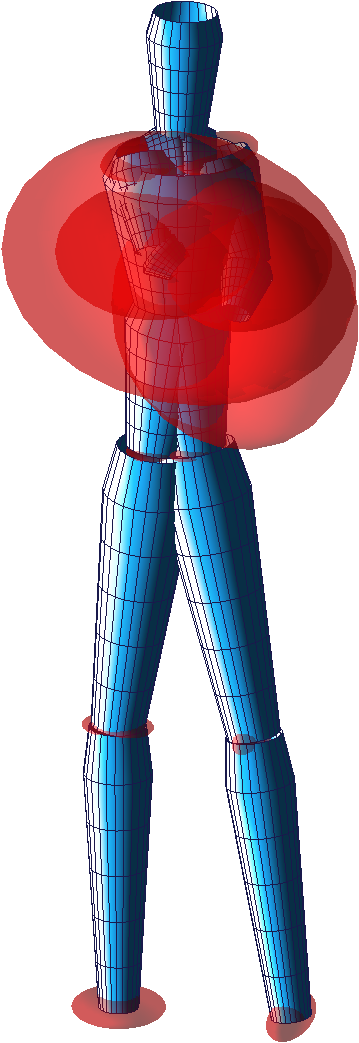
\includegraphics[height=0.135\linewidth]{fig/poseest/APE/boxxerr.png}

\end{tabular}
\caption{3D pose estimation results with different action classes from the APE dataset: (left) Detected 2D parts and bounding box from action detection (right) the 3D pose estimated.  Red ellipsoids represent the confidence region of pose estimation, $\finalvariance$, in equation (\ref{eq:combination2}). Sample (o) and (p) shows the wrong pose estimations when the 2D body part detector fails.}
\label{fig:aperesults}
} 
\end{center} 
\end{figure*} 
